\documentclass[twoside]{utmthesis}
%According to the new manual, should not mixed single-side with two-side printing

\usepackage{graphicx}
\usepackage{url} 
\usepackage[pages=some]{background}
\usepackage{natbib}
\usepackage[T1]{fontenc}
%\let\cite\citep
\let\cleardoublepage\clearpage
\usepackage{lipsum}
\usepackage{enumitem}
\usepackage{pdflscape}
\usepackage{float}
\usepackage{mathtools}
\usepackage{lscape}
\usepackage[figuresleft]{rotating}
\usepackage[justification=centering]{caption}
\usepackage[per-mode=fraction]{siunitx}
\usepackage{fancyvrb}

\begin{document}

% Required information
\title{News Event Prediction using Causality Approach}
\titletwo{on South China Sea Conflict}

\author{TEO WEN LONG}
\degree{Bachelor Degree of Computer Science}
\specialization{Network and Security}
\intakeyear{2016}
\school{School of Computing}
\faculty{Faculty of Engineering}
\titledate{January 2019}
\award{1}
% Options for Award 
% 1. Bachelor Degree Project Report
\superone{Dr. Anazida Binti Zainal}


% Mandatory pages
\coverpage
\superpage
%\certification
\frontmatter
\maketitle
\declaration

\begin{dedication}
This thesis is dedicated to my family, for their endless support in the success of my degree study. It is also dedicated to my beloved friends who taught and guide me throughout the project.

\textit{"Shoot for the moon, even if you missed, you'll land among the stars."} 
\end{dedication}

\begin{acknowledgement}
First of all, I am grateful to my family for always backing me up during my degree study. I would like to express my warm appreciation and sincere thanks to them. No words can express my thankfulness to them.

I would also like to thank to my supervisor, \textbf{Dr. Anazida bt Zainal} for her patient and willing to teach. She is one of the best supervisor that always guide me whenever I faced with difficulties in the project. She also inspired me the beauty of data analysis and explore me with different techniques and platform that benefits to me throughout my study. 

Besies, I would like to thank the authority of Universiti Teknologi Malaysia (UTM) for providing me with excellent equipment and study environments such as Students Lounge, High-speed WiFi, etc. Time spent in UTM is never wasted. 

Last but not least, Thank you. To all the people I love.   
\end{acknowledgement}


\begin{abstract}
South China Sea (SCS) is one of part from Pacific Ocean where generate huge economic value in fishing and shipping lane as well as high amount of natural resource. Various countries such as China, Vietnam, Philippines, Taiwan, Malaysia and Singapore surround SCS. Due to the strategy location of shipping lane and high revenue generated, SCS become place where several nearby countries compete for its territorial claims. Famous territorial disputes such as Spratly islands, Paracel island, Scarborough Shoal were happened for the claims of the wealth on SCS. To reflect these issues, newspaper are the main medium that propagate the first-line message to the public and update whenever there is SCS conflict happened. Within news events occurred, there are causal relation between cause and effect that able to obtain and analysis for the trend of event happening. This is known as causality in news article. Besides,in order to avoid any inevitable tragedy happen within SCS conflict, event prediction is important as it gives a better insight and foresee future events that might happen. Event prediction is a technique to measure the trend of happening events and forecast upcoming events that might happen. In this project, abstract event causality network proposed by \cite{zhao2017constructing} will be used as prediction model and furthermore embed the causality network into a continuous vector space.It is used because of its general, frequent and simple causality patterns as well as simplify event matching that suitable for event prediction. First, it extracts news article based on causality connector such as "because", "after", "lead to", etc into <cause, effect> tuple. Then, it represents the tuple with noun-verb representation and further generalised using WordNet and VerbNet. After that, an abstract causality network is build by using frequently co-occurring word pairs (FCOPA) and further embed into a continuous vector space for simplifying event manipulation while preserving cause-effect structure of the original network.    
\end{abstract}

\begin{abstrak}
Laut China Selatan (SCS) adalah sebahagian daripada Lautan Pasifik yang menghasilkan nilai ekonomi yang besar dalam memancing dan lorong perkapalan serta jumlah sumber asli yang tinggi. Pelbagai negara seperti SCS, China, Vietnam, Filipina, Taiwan, Malaysia dan Singapura. Disebabkan lokasi strategi lorong perkapalan dan pendapatan tinggi yang dihasilkan, SCS menjadi tempat di mana beberapa negara berdekatan bersaing untuk tuntutan wilayahnya. Pertikaian wilayah yang terkenal seperti pulau Spratly, pulau Paracel, Scarborough Shoal telah berlaku untuk dakwaan kekayaan di SCS. Untuk menggambarkan isu-isu ini, akhbar adalah medium utama yang menyebarkan mesej baris pertama kepada orang ramai dan mengemaskini apabila terdapat konflik SCS. Di dalam kejadian berita berlaku, terdapat hubungan kausal antara sebab dan akibat yang dapat diperoleh dan analisis untuk trend kejadian yang berlaku. Ini dikenali sebagai kausalitas dalam artikel berita. Selain itu, untuk mengelakkan sebarang tragedi yang tidak dapat dielakkan berlaku dalam konflik SCS, ramalan peristiwa adalah penting kerana ia memberikan wawasan yang lebih baik dan meramalkan peristiwa masa depan yang mungkin berlaku. Ramalan acara adalah teknik untuk mengukur trend peristiwa yang berlaku dan meramalkan peristiwa akan datang yang mungkin berlaku. Dalam projek ini, rangkaian kausal sebab abstrak yang dicadangkan oleh \ cite {zhao2017constructing} akan digunakan sebagai model ramalan dan seterusnya membenamkan rangkaian kausal ke dalam ruang vektor yang berterusan. Ia digunakan kerana corak kausal yang umum, kerap dan sederhana serta memudahkan pemadanan acara yang sesuai untuk ramalan peristiwa. Pertama, ia mengeluarkan artikel berita berdasarkan penyebab kausal seperti "kerana", "selepas", "membawa kepada", dan lain-lain ke dalam <cause, effect> tuple. Kemudian, ia mewakili tuple dengan perwakilan kata nama-kata kerja dan lebih umum menggunakan WordNet dan VerbNet. Setelah itu, rangkaian kausal abstrak dibangunkan dengan menggunakan pasangan kata sepasang yang lazim (FCOPA) dan memasukkan lebih lanjut ke ruang vektor yang berterusan untuk memudahkan manipulasi peristiwa sambil memelihara struktur sebab-akibat rangkaian asal.
\end{abstrak}


\tableofcontents
\listoftables
\listoffigures


%List of abbreviation 
\listofabbre
\newline
\addabbre{SCS}{South China Sea}
\addabbre{ORG}{Organisation}
\addabbre{LOC}{Location}
\addabbre{GPE}{Geographical Entity}


%List of symbols 
%\listofsymbols
%\addsymbol{$SIM(e_{i},e_{j}) = f(dist_{Gen}^{G_{p}}(P^{i},P^{j}),dist_{Gen}^{G_{o}}(O_{1}^{i},O_{1}^{j}),....,dist_{Gen}^{G_{o}}(O_{4}^{i},O_{4}^{j}))$}{2.1}

%\addsymbol{$\sigma$}{Whatever}
%\addsymbol{$\varepsilon$}{Whatever}


%Uncomment if have appendices
\listofappendices


\mainmatter


\chapter{Introduction}


\section{Overview}
Newspaper is an important part of our life as it is a printing media in which all information of either national or international news are published and delivered to the public every day. Henry Ward Beecher (1887), an American social reformer and well-known speaker once said, “Newspaper is a greater treasure to people than uncounted millions of gold.” Articles within the newspaper play essential role in education development and makes public aware about events happening in the region or nation that they are living in. By reading newspaper, readers can learn and observe others point of view as it brings another whole new perspective on same events. In the digital era, artificial intelligence (AI) expert make use of the digital technologies to get a better insight within the traditional media, newspaper.\cite{jamesbaker2019} Within these digital technologies, event prediction held a big portion as it forecast future events and it is valuable to alert public on predicted events. 

Event prediction is a data analytic technique that make use of experience and knowledge as well as pattern from past to predict future events. Natural disaster prediction is one of the examples in applying concept of event prediction. For example, Japan is a well-known earthquake active country as its archipelago is in an area where multiple continental and oceanic plates collapsed together. Hence, earthquake forecasting is important for Japan and scientific report \citep{jamesd.goltz2018} stated that earthquakes cluster in time and location as it can be predicted and take precaution before tragedy happened. Besides, event prediction is also useful in business intelligence. A report in 2016 also showed that business analysis and prediction help them to understand more about their customer, in order to enhance the success of their marketing strategies. \citep{erevelles2016big}

Every country had its obligation to protect its national security. National security is a requirement to maintain the survival of a country though economic, diplomacy, political and ethical power and focus on freedom from military threat and political coercion. Without national security, a country might at risk and attacks such as terrorism, sabotage, information warfare, etc might infiltrate the country. For example, ISIS threat stunned the world as a gunman, Mehdi Nemmouche opened fire at Jewish Museum of Belgium in Brussels as he is suspected in joining extremist groups, ISIS in Syria. This event took 4 lives of innocents.\citep{rafcasert}

South China Sea (SCS) is a conflict zone whereby an estimated USD5 trillion worth of raw products shipped through shipping lanes in SCS each year and its nearby countries made them fight over each other to have the main control of the whole SCS. \citep{theNationalInterest} The conflict is known as South China Sea disputes. The events of territorial disputes of South China Sea populated all the newspapers and many events regarding to the disputes were reported through national news agency. It rises concerns about the beginning of world war as for example a near-collision between US warship, Decatur and Chinese Luoyang missile destroyer in South China Sea highlights the escalating danger of confrontation between US and China. (Ni, 2018) SCS is strategically located at peripheral ocean that is a piece of the Pacific Ocean, starting from Karimata and Malacca Straits to the Strait of Taiwan with area about \SI{3500000}{\km\squared}.Besides, South China Sea is rich in marine life and natural resources such as oil and natural gas, even have the most of the important shipping lanes in the world. \citep{dennise.hayes1980}

Causality is the relationship between cause and effects. Every event will occur first on cause and followed by effects. In SCS disputes, causality is highlighted between benefits from SCS (cause) and territorial disputes (cause) is clearly highlighted in SCS disputes events.
	
In order to have an advanced insight among these disputes, event prediction is necessary, and causality should be taken as main attributes. However, there are still several problems and challenge to be solve in order to achieve an excellent prediction model based on causality.  


\section{Problem Background}
National security is always the top priority of governments to protect society from disruption owing to a disaster or crisis. There are many aspects on national security such as territorial, economic, physical, social, political etc. However, the peaceful of national security had been affronted by South China Sea disputes. 

Due to geological and resources advantages of South China Sea, countries within the region such as Brunei, China, Taiwan, Malaysia, Indonesia, Philippines, Vietnam etc. made competing the territorial claims over it. Based on news on The National Interest in 2016, an estimated US 5 trillion worth of global trade passes through the South China Sea annually. Hence, territorial disputes in the South China Sea started to concern worldwide community about peace of world. In order to claim the ownership of South China Sea, countries are challenging against each other by putting military force in the area. This can be observed from the news of China spent almost 1 year to build 7 new islands by moving sediment from the seafloor to reefs and after that focused on building ports, airstrips and other military structures on the islands. 

South China Sea dispute had a brief background involving timeline from 221 BC until recent. Each of the historical event occurs and accumulates and eventually things go haywire. Many dispute events happened in either small or large scale. For example, Spratly island dispute \citep{gonzales2014spratly} and “nine-dash” line  \citep{liuzhen2014} that proposed by China is some of the significant disputes in South China Sea. Besides than these two issues, there are many issues that remain unsolved and will constantly concerning the worldwide community. 

However, all the information retrieved from news article are unstructured. Unstructured data have no recognizable structure via pre-defined data models and schema and mainly generated by human or machine. \citep{christinetaylor2018}. By collecting these unstructured data from the past and analysing its trends, we are able to have a better understanding about what may happen in the future. \citep{bryanbell2016}. In SCS disputes, event prediction is important to give public a better understanding about future events that might happen. A better policy can be made with regards to protect national security under SCS disputes with the event prediction technique based on unstructured data in news articles. 

In event prediction based on news articles, there may have some challenges. First, news article is a type of unstructured data that contain a lot of valuable information in term of cultural, social and historical \citep{yzaguirre2016newspaper} but doesn't fit into traditional row and column structure of relational databases.\citep{mongoDB2016}. It require substantial manual effort to analyse and extract the essential information from news articles. Second, a event that causes another events may completely different from the real prediction. It is indicating that the predictive model provides a faulty outcome that hard to distinguish from the true prediction. 

There are several researchers research on topic event prediction with different method. Granroth-Wilding (2016) proposed a predictive neural network model that learns embeddings for words describing events, a function to change embeddings into event representation and a function to predict the degree of relationship between two events.However, the model is more focus on chain or events sequence which is good for rich-infomrative events but might not suitable for news articles that have unordered sequence. Preethi (2015) proposed an event prediction model for Tweets using temporal sentiment analysis and causal rules extraction. This model is useful to analyse user's sentiments and predict future events using temporal attribute. This study analyse sentiments of user's opinion and is not suitable for news articles whereby formal news reports seldom express their sentiments within the articles. 

\cite{zhao2017constructing} proposed an abstract event causality networks based on causality attribute. The predictive model is suitable for unstructured data such as news article and learn from previous events to predict the future. Given a South China Sea events stated that "Vietnam started to protest for their sovereignty in South China Sea because of China construct a new military purpose platform on strategically-located Bombay Reef in South China Sea." From this event, causality connector "because of" is identified and cause-event pair is extracted based on the pattern of effect <because> cause. The causality pair is then further simplified and generalise by verb-noun representation as well as WordNet and VerbNet and further take a part in constructing abstract event causality networks. 


\section{Problem Statement}
South China Sea (SCS) is a conflict zone where events happened from time to time with different severity. This greatly impact or influence the policy that made by government of Malaysia to overcome the negative impacts brought by SCS territorial disputes in term of national security. The problem is to extract valuable information from SCS conflict events and predict the future events that may happen. Besides, online news is unstructured data and extracting correct information from massive online news articles that contain different resources automatically is part of the challenges. Event prediction is biased to measure, and a good predictor is needed to make sure that its prediction is accurate and precise.    

\section{Aim/Purpose of Study}
This study will address the SCS disputes issues by implementing \cite{zhao2017constructing}'s abstract event causality network and its embedding model. This model learns causality of events and provides simplify event matching which is advantage for event prediction. 

\section{Research Question} 
\begin{enumerate}
	\item How to obtain useful information from news article that related to South China Sea conflict?
	\item How to generalise and cluster extracted event pairs and how to relate event pairs with causality?
	\item How to use the extracted information to train and build a prediction model?
\end{enumerate}

\section{Objective}
\begin{enumerate}
	
	\item To extract <cause, effect> causality pairs from news articles in South China Sea conflict by using causality connectors
	
	\item To extract all important information from causality pairs by using verb-noun representation as well as discover general patterns using WordNet and VerbNet.  
	
	\item Train and build an abstract causality network with frequently co-occurring word pairs (FCOPA) and embed the model into a continuous vector space.
\end{enumerate}

\section{Scope} 
Event prediction is important to have better understanding for future event that may happen, but it also have its limitations that need to address and narrow down. Below are the scope of this study:-

\begin{enumerate}
\item The coverage of this study will be using news articles that extracted related to SCS conflict only. 
\item The study will focus on SCS conflict news from online news article that having keywords related to SCS. 
\item The study will only covers the some of the causality connectors such as "because of", "because", "after", "due to", etc.
\item Prediction model in this study will be based on abstract causality network from \cite{zhao2017constructing}
\end{enumerate}	

\section{Significant of Study}
Event prediction is important because it give a better insight and forecast for public about events that possible to happen. Besides, in SCS conflict, event prediction can be used to protect national security of Malaysia and appropriate actions can be took by governments to prevent the happening of unseen tragedy based on predicted events. In addition, Malaysia governments are able to protect the sovereignty of country in SCS region to claim peace and avoid involving in SCS conflict.    

\section{Organisation of Study}
\textbf{Chapter 2} will be discussed the literature review of event prediction and information extraction from news articles based on different method and referenced method. \textbf{Chapter 3} will focus on research methodology, research framework, overall research phase, as well as measurement and rules.  \textbf{Chapter 4} will be present about initial result of implementing prediction model proposed by \cite{zhao2017constructing} by on step-by-step approach with causality attributes. \textbf{Chapter 5} will be summarised work done in PSM 1 and discussed future works involving in this project.


% Chapter 2

\chapter{Literature Review}

\section{Introduction}
This chapter will discuss the literature review of event prediction using causality approach on South China Sea (SCS) conflict. First, the chapter will briefly explain about event prediction and SCS conflict Then,the chapter will discuss text mining which consists of many stages such as text preprocessing, event extraction, event representation, event generalisation and event relation. After that, this chapter will briefly discuss the prediction algorithm and justify the most suitable algorithm for SCS conflict event prediction in this paper. Finally, this chapter will compare existing work that had done in the domain of event prediction. Last but not least, this chapter will discuss  open issues in event prediction that need to be addressed, followed by a short brief summary.  


\section{Event Prediction}
Event prediction is a technique to measure the trend of happening events and forecast upcoming events that might happen. According to Cambridge dictionary, event stands to anything that happens especially something important or unusual while prediction is a statement about what you think will happen in the future. Figure 2.1 shows a taxonomy of event prediction. The taxonomy is sketched based on generic steps needed to be performed in event prediction. Steps such as text preprocessing, event extraction, event representation etc. is important in the progress of building up a successful predictive model. The main part of event prediction is text mining which will be further discussed in the following section.  

\begin{figure}[H]
\centering
\fbox{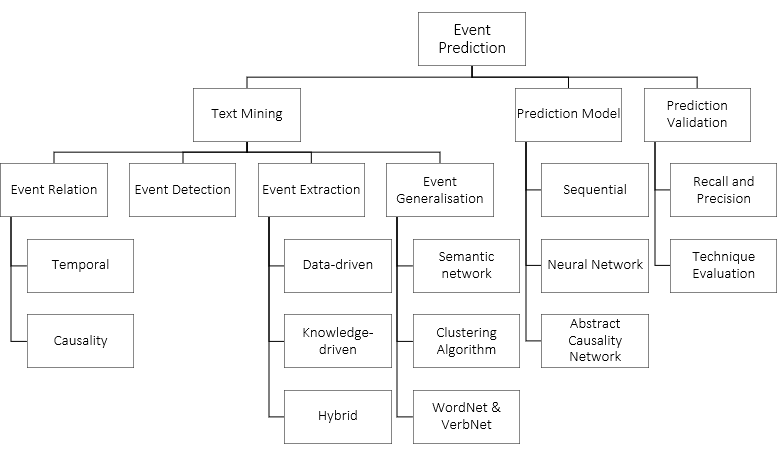
\includegraphics[width=1\textwidth]{./diagram/taxonomy}}
\caption{Taxonomy of Event Prediction - Generic steps needed to performed in event prediction}
\end{figure}  
\vspace{-1cm}
 
Event prediction involves in many domains. Research on areas of event prediction are active and wide. Example of domains in event prediction are below:
\begin{enumerate}
	\item Natural disaster such as earthquake \citep{asencio2017medium,asim2017earthquake} and tsunami \citep{mulia2016real},
	\item Political such as election prediction \citep{tung2016mining}
	\item Social such as protest event in Argentina  \citep{ning2016modeling}
	\item Economics such as predicting market stock price \citep{ding2015deep,vargas2017deep}, etc.  
\end{enumerate}

In news articles, there are many events happen everyday. From political issues, to social problems, economic trend and entertainments, newspaper provides public daily updates on these events. Recently, conflict happened on South China Sea (SCS) has becoming popular and continuously escalated. The happening of SCS conflict concerns countries nearby the regions and it must be solved and actions should be taken to prevent happening of any tragedy.     

If there is no such the problem or the conflict in the South China Sea, we no need to carry out the research to find out the way to extract the causality from the news articles and predict the effects. This is because of the stupid countries want to fight for the lands and the sea areas.

\section{South China Sea Conflict}
South China Sea (SCS) is located strategically within Asia countries such as China, Taiwan, Indonesia, Philippines, Vietnam, and Malaysia. It has the busiest shipping lane as one-third of world's shipping passes through SCS and almost 3.37 trillion global trade happened within SCS in year 2016  \citep{chinapower2016}. Due to these huge market profit, many countries started to claim that SCS is their own territory and China even illustrated a "nine-dash line" which is a huge part from SCS and claim that region within "nine-dash line" is China's territory \citep{liuzhen2014}. These started the dispute between countries. For every dispute, public are able to know the flow of events through newspaper.

Examples of famous SCS dispute are Spratly islands dispute and China-Vietnam Military Clash. Spratly islands covered with huge amount of natural resources, global maritime areas and commercial shipping lane. In year 2015, China had militarised Fiery Cross Reef, reef located at the western edge of SCS and centre of Spratly islands by constructing military-level airstrip and seaport. This made concerns to Vietnam and Philippines as they felt threaten to their sovereignty in SCS region. Besides, China and Vietnam are continuously declared their ownership in SCS on oil and gas exploration issues. The issues are escalating as reports \citep{vietnamBoat2014} showed that Vietnam tried to ram Chinese vessels in SCS dispute area.     
 
New articles are written by different news agency with different perspective and opinion.Among many of the newspaper agency, National news agency such as Xinhua News Agency for China and Vietnam New Agency (VNA) are said to be the voice of government. \cite{gautierbattistellaOctober2005} stated that Xinhua is the biggest propaganda machine that spread the core concept of China's government to the public. Hence, there are huge amounts of valuable information that represent and reflect the action of government can be obtained within  news article from national news agency. However, without proper technique to extract useful information from the news article, the data source will be difficult to be obtained and time-wasting. In the next section, text mining will be introduced as an effective method to obtain valuable information from the news articles.   


\section{Text Mining}
Text mining, also known as knowledge discovery from textual databases and related with steps of obtaining valuable and non-trivial pattern or knowledge from unstructured text documents \citep{tan1999text}. A general framework proposed by \cite{tan1999text} in Figure 2.2 shows text mining contain two major elements, which are text refining and knowledge distillation. Text refining are techniques to transforms free-form text into intermediate form meanwhile knowledge distillation is to obtain the pattern or knowledges within the intermediate form. From text refining, two types of intermediate form can be obtained, document-based or concept-based which are able to be further processing into visualisation or predictive modelling.   

\begin{figure}[h]
\centering
\fbox{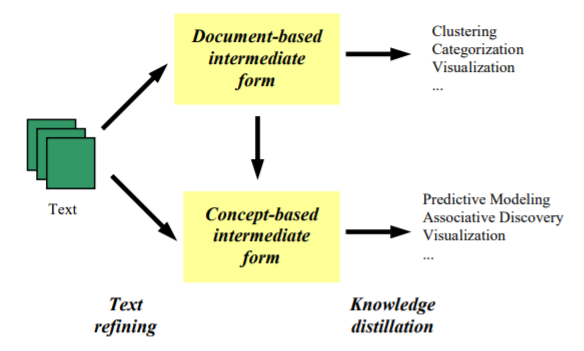
\includegraphics[width=1\textwidth]{./diagram/textMining}}
\caption{General Text Mining Framework proposed by \cite{tan1999text}}
\end{figure}

However, there are open problems in text mining that need be addressed. For examples, variety of intermediate form that causes complexity and uncertainty in text mining, multilingual text refining, domain knowledge integration \citep{lima2009domain}, and customized autonomous mining \citep{afzal2010rule}.

\pagebreak
\subsection{Types of Data}
With text mining, useful information can be extracted for further processing. However, the volume of data is dramatically increasing nowadays, associated with high flow of data and high variety of information. For example, inside a single webpage, different type of data such as images, audio, textual data, comments, etc. can be obtained and categorised. Two major categories of data are structured data and unstructured data. Both of the categories will be further discussed in the following sections. 

\subsubsection{Structured Data}
Structured data is referred to the data that organisation all the information in formatted way and easily to extract and analysis by relational databases\citep{christinetaylor2018}. Example of structured data are phone number, name, identification numbers, date,etc. Format of structured data is analysable with human-generated queries and algorithm.  

\subsubsection{Unstructured Data}
Unstructured data is referred to the information that does not have a pre-defined model or structure and unable to store in traditional relational databases. Example of unstructured data such as text, emails, blogs, web pages, images, audio, comments on social media, etc. has no proper structure and has to be processing into valuable information before analysing them. Figure 2.3 shows the example of structure data(numerical and statistical data) and unstructured data(text, audio, video and blog posts).
\begin{figure}[H]
	\centering
	\fbox{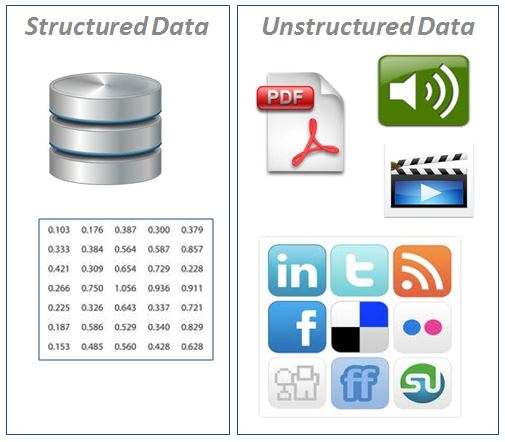
\includegraphics[width=0.7\linewidth]{diagram/Unstructured-Data-Examples}}
	\caption{Example of structured and unstructured data \citep{michaelbenzmoritzmuller}}
	\label{fig:unstructured-data-examples}
\end{figure}
\vspace{-1.5cm}

Nowadays, unstructured data is getting enormous. Information contained within these unstructured data originating from humans is absolutely richer and more valuable than traditional numeric data sources \citep{FRUNZA2016263}. Besides, study in 2019 \citep{rohitbigdata2019} showed that 95 percent of businesses need to manage unstructured data and more than 150 zettabytes(150 trillion gigabytes) of data will be needed for analysis by 2025. Because of that, exploring and extracting useful information from these unstructured data is essential. However, text mining is difficult due to ambiguity of languages, multiple duplicated words with different meanings, abbreviation, linked references etc\citep{bhardwaj2016text}.To overcome the difficulties, many techniques such as Named Entity Recognition (NER), Nature Language Processing (NLP), sentiment analysis, causality relationship extraction etc. are developed to extract high quality information from textual data. 

News event from SCS conflict is one of the unstructured data which the textual data is raw and does not have a proper structure on the sentences. Hence, further processing for the news events is important and it should be started with text preprocessing. 

\subsection{Event Relation}
Event relation is important in text mining as it provides better insight and understanding about event happens either before or after. Generally, there are 2 major type of event relation that can be observed and obtain from news article which are temporal relation and causality relation. As events happen from time-to-time, temporal attribute should be focused as it measures the trend and evolution of event. Besides, there is always a cause for events to happen, hence causality is used to relate events from the very beginning based on its cause.

\subsubsection{Temporal Relation}
Temporal is indicated as time-based or using time as the main measurement. Usually, events getting worse from a small case. For example, in medical domain, long-term follow-up is important for medical investigation. \cite{maziarz2017longitudinal} make use of temporal relation to observe the trend of patient's health condition over time, and eventually predict patients' risks for a future adverse outcome. Besides, temporal relation had been widely adopted in event prediction with different domain such as micro-blog and tweets \citep{preethi2015temporal}, sports \citep{grolinger2016energy}, stock market flow \citep{ding2015deep} and etc. 

\subsubsection{Causality Relation}
The main concept of causality is that one or more things/events as causes can cause one or more things/events to happen as effect. In news article, there are many events that related with each other but hard to be observe and detect by human or massive news events happen in the same time cause human hard to digest all the news happened in one time. Thus, people tend to automated the extraction of news article based on causality. However, there are many challenges in automating the process. For example, \cite{pechsiri2010explanation} faced difficulties on explanation knowledge graph through causality extraction from text such as causal-boundary determination and effect-event pattern determination. Nevertheless, it is useful for event extraction because it contain cause and effect that allows people to understand more about the following events. In this study, we will focus on causality relation as SCS conflict happens after certain small case instead of following time flow.  

\begin{enumerate}
	\item \textbf{Causality Pair}
	
	Causality pair is also known as entity pair, used to represent causality within pairs. For instance, \cite{mirza2014extracting} stated possible causality pairs in his study as (1) main events of consecutive sentences, (2) pairs of events in the same sentence, (3) an event and a time expression in the same sentence. If the pairs are tagged as (\textit{e\textsubscript{1},e\textsubscript{2}}), the pairs will be \textit{events-events}, \textit{events-timex}, \textit{timex-timex}. 
	
	\item \textbf{Causality Rules}
	
	After identify the potential cause-effect pairs, it is difficult to execute human-annotation on these causality pairs as the amount of data is getting enormous. Hence, autonomous annotation is proposed. 	In the work of \cite{radinsky2012learning}, Radinsky use causality rule to predict the future event as abstraction tree (AT) had been build earlier and using causality rules, a causality graph is built to explain the predicted event clearer.
	
	Moreover, in order to get an accurate categorised result based on causality pair, causality rules is set in every text extraction. \cite{zhao2017constructing} construct a set of causality rules that follows the template of <\textbf{Pattern,Constraint,Priority}> where Pattern indicates the trend of events between causality pairs, Constraint indicates the limitation on sentence which the pattern can be applied, Priority indicates the priority of causality pairs to be execute first or second. After extracting causality pairs from news article as well as generalise for more general purpose, an abstract causality network is built. 
	

	
	\item \textbf{Causality Network}
	
	Causality network is a path diagram that visualise the causal relationship between events and enable researchers to estimate effects sizes and costs \citep{dahlhaus2003causality}. Generally, Granger causality is widely used in causality network for event prediction model as it is a statistical concept of causality. \citep{Seth2007}. In Granger causality, a true cause-and-effect relationship is obtained from particular variable that comes before another and it used bottom-up approach to predict the outcome. 
	In \cite{zhao2017constructing}, causality network is separated into 2 parts, abstract causality network and specific causality network in which mentioned in Figure 2.4. In Figure 2.4, an abstract causality network is built on top on specific one, where the node of abstract causality network are frequently co-occuring word pairs, which are general enough for representing event trend. 
	 
	\begin{figure}[H]
		\centering
		\fbox{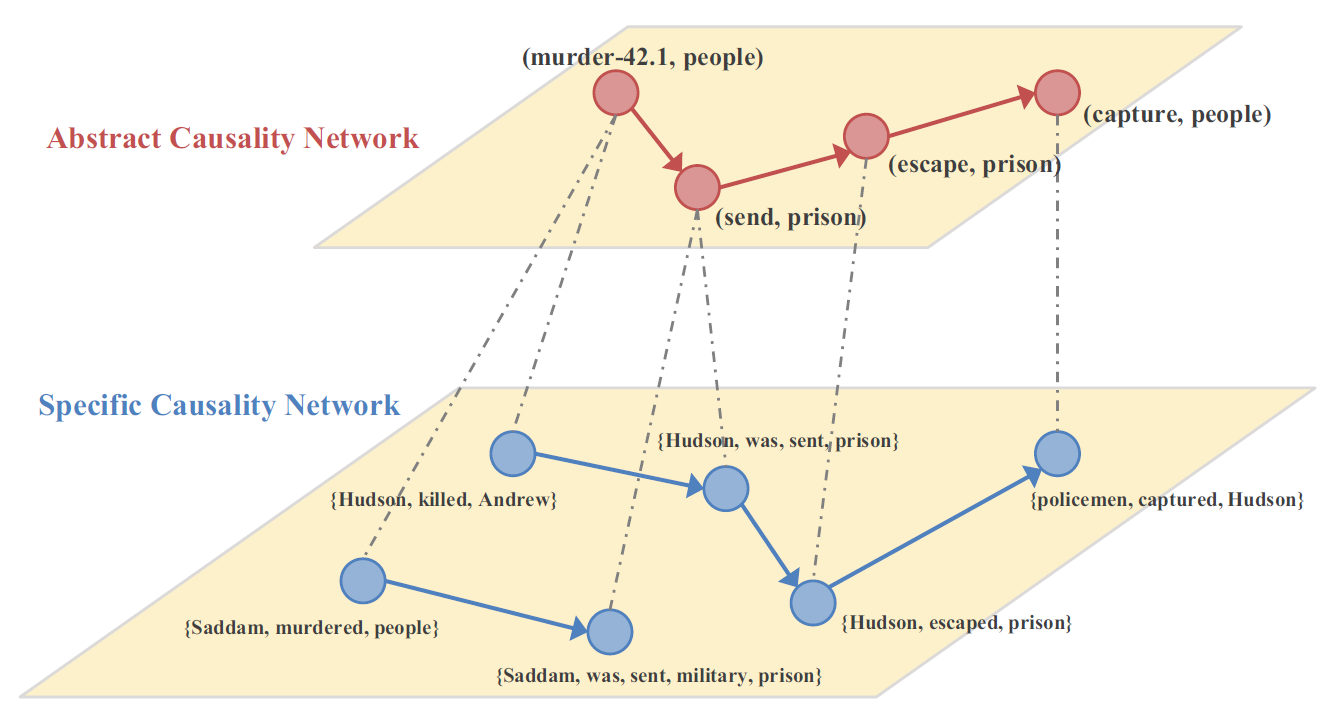
\includegraphics[width=0.8\textwidth]{./diagram/causality_network}}
		\caption{Example of Causality Network, adopted from \cite{zhao2017constructing}}
	\end{figure} 
	\vspace{-1cm}
\end{enumerate}

\subsection{Event Detection}
Event detection is a techniques to discover occurrences of events by analysing text stream in the sources. Generally, event detection can be broadly categorised as either feature-pivot (FP) or document-pivot(DP) \citep{fedoryszak2019real}. Based on \cite{chen2019bibliometric}, feature-pivot is the method that detecting abnormal patterns in appearance of features such as words. When an event happens, the frequency of a feature will be abnormal comparing to its unusual behaviour which indicating a potential new event. Meanwhile, document-pivot is using documents as items to clustered them by using similarity measure. 




\subsection{Event Extraction}
Event extraction is one of the common application of text mining as it obtains specific knowledge concerning incidents referred to texts \citep{hogenboom2011overview}.  Figure 2.6 shows the general procedure of event extraction. Event extraction uses data that are preprocessed using the methods mentioned in the previous chapter, and further represent by general causality pairs. Moreover, event relation is determined to have a better insight between events.  

\begin{figure}[H]
	\centering
	\fbox{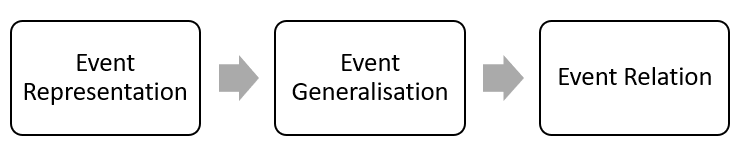
\includegraphics[width=0.7\linewidth]{diagram/eventRepresentation}}
	\caption{General procedure of event extraction}
	\label{fig:eventrepresentation}
\end{figure}
\vspace{-1.5cm}

Based on report by \cite{hogenboom2011overview},there are three main approaches to event extraction, which are data-driven, knowledge-drive and hybrid. \cite{hogenboom2016survey} performed an investigation based on these three approach by surveying their usage in different domain. Three of the approaches will be further discussed in the subsections below. 

\subsubsection{Data-Driven Event Extraction}

Data-driven approach is mainly used for natural language processing (NLP) application and focus on quantitative methods. It focuses on converting statistics data into knowledge. Data-drive approach is not restricted to fundamental statistical reasoning but maximize the quantitative measure for automated extraction. One of the weakness in data-driven approach is that it doesn't consider about meaning and sentiments and require a large amount of data to get statistically significant results.

\subsubsection{Knowledge-Driven Event Extraction}

Compared to data-driven, knowledge-driven is more focus on patterns and exploring human-knowledge. It considers sentiments and consumes less training data compared to data-driven, and also able to define powerful expression by using semantic elements for an easily interpretable and traceable result. Most common pattern extracted are lexicon-syntactic pattern and lexicon-semantic pattern. Both of the patterns are based on lexicon normalisation and must be deployed on preprocessed data. However, knowledge-driven requires more advanced expert knowledge and more difficult to extract due to the challenge of language ambiguity and pronoun resolution that might occur in lexicon.  

\subsubsection{Hybrid Event Extraction}

In order to balance both advantages and disadvantages between data-driven and knowledge-driven extraction, hybrid approach is used to overcome the lack of expert knowledge in pattern-based problem, by applying statistical methods. For advanced extraction techniques, hybrid approach is prioritised in order to optimise the difficulties level in knowledge-drive approach and huge amount of data in data-driven approach. 

Event extraction is still under active research and researcher tend to produce a best solution for all the problems and challenge obtained in event extraction. Table 2.1 shows the comparison of recent research on event extraction. By comparing some research, it can be concluded that if the model has large corpus, data-driven approach will be used. Meanwhile, if the model require rule-based extraction, knowledge-driven approach is needed. In this study, hybrid approach is used because there are large corpus on news events and require some simple rules to extract events precisely.  

\begin{table}[H]
\fontsize{11}{12}\selectfont
\caption{Comparison of Recent Research on Event Extraction}
\renewcommand{\arraystretch}{1.2}
\begin{tabular}{|p{2cm} |p{4cm} |p{2cm}|p{5cm}|}
	\hline 
	Author, year & Domain & Approach & Limitation \\ 
	\hline 
	\citep{wu2017event}&Event Timeline Extraction on News Corpus &Data-driven  & Require large text corpus \\ 
	\hline 
	\citep{valenzuela2015domain}&Domain-independent Rule-based Framework for Event Extraction  & Knowledge-driven & Needs to design multiple rules for different domain  \\ 
	\hline 
	\citep{rospocher2016building}& Building event-centric knowledge graphs from news & Hybrid & Expert knowledge required to build knowledge graph \\ 
	\hline 
	\citep{vossen2016newsreader}&Using knowledge resources in cross-lingual reading machine from news  & Hybrid & Require knowledge acquisition and NLP improvement on a massive scale \\ 
	\hline 
\end{tabular} 
\end{table}
\vspace{-1cm}

\subsection{Event Representation}
After extracting useful information from event extraction techniques, these data is match with certain meaning to represent certain knowledge.  In work of \cite{ding2015deep}, Stanford Open IE, a Java-based information extraction application is used. In Open IE, it first use ReVerb \citep{ReVerb2011} ,a autonomous program that identifies and extract binary relationship from English sentences with tuples of event, then use ZPar \citep{zhang2011syntactic} to parse the sentence with subject, object and predicate. The event is represented as tuple \textit{E = (O\textsubscript{1},P,O\textsubscript{2},T)}, where O\textsubscript{1} is the actor and O\textsubscript{2} is object, P is the action and T is the timestamps of the event. In this project, works of \cite{zhao2017constructing} will be referred as it represents event causality will a more simpler and straightforward method. By using regular expression mentioned earlier, event is represented as \textit{<cause, effect>} pairs 

Event representation using tuples is widely used with different domains in different paper. Table 2.2 shows some research that are using tuple approach in different domain such as social media and economic. By the best of our knowledge, almost all the event representation are using tuple approach but with different attributes arrangement and consideration. By using tuples, it provides clearer picture of the event and easier to categorise each element in tuple with their corresponding category. 

\begin{table}[H]
	\fontsize{11}{12}\selectfont
	\caption{Research done in Event Representation}
	\renewcommand{\arraystretch}{1.2}
	\begin{tabular}{|p{3cm} |p{4cm} |p{7cm}|}
		\hline 
		Author, year & Domain & Representation \\ 
		\hline 
		\citep{anantharam2015extracting}&Extracting city traffic events from social streams & <e\textsubscript{type},e\textsubscript{loc},e\textsubscript{st},e\textsubscript{et},e\textsubscript{impact}> where represent type of event, location, smallest timestamp, largest timestamp and impact of event respectively \\ 
		\hline 
		\citep{zhou2015unsupervised}&Unsupervised framework of exploring events on twitter  & <\textit{y,d,l,k}> where represent non-location named entities, date, location and event-related keywords respectively \\ 
		\hline 
		\citep{ding2016knowledge}& Knowledge-driven event embedding for stock prediction & \textit{E = (A,P,O)}, where P is the action or predicate, A is the actor or subject and O is the object on which action is taken \\ 
		\hline
		\citep{radinsky2012learning} & Event prediction based on causality & \textit{e = <P,O\textsubscript{1},....,O\textsubscript{4},t>}, where P is the events' objects, O\textsubscript{1} to O\textsubscript{4} is the actor,object,instrument,location and t is timestamp \\
		\hline
	\end{tabular} 
\end{table}
\vspace{-1.5cm}

\subsection{Event Generalisation}
Generalisation on causality pattern is very useful in discovering high-level causality rules behind specific causality pairs \citep{zhao2017constructing}. It is an important step after event extracton and representation since the model structure is unclear and may have duplicate and similar event pairs that increase the difficulties in text processing. For example, an event "\textit{a massive 8.9-magnitude earthquake hit north-east Japan on Friday}$\,\to\,$\textit{a large amount of houses collapsed}" can be generalised into \textit{earthquake hit}$\,\to\,$\textit{house collapse}. The generalisation method helps to eliminate unnecessary words to ease the text processing. 

Besides, \cite{radinsky2012learning} utilised the concept of generalisation by finding the similarity between two events e\textsubscript{i} and e\textsubscript{j} by applying a function of distances between objects and actions: 
\begin{equation}\label{2.1}
SIM(e_{i},e_{j}) = f(dist_{Gen}^{G_{p}}(P^{i},P^{j}),dist_{Gen}^{G_{o}}(O_{1}^{i},O_{1}^{j}),....,dist_{Gen}^{G_{o}}(O_{4}^{i},O_{4}^{j}))
\end{equation} 
where $dist_{Gen}^{G_{p}}$ is the distance function in graph and f is an aggregation function. By finding the similarity between two events, generalisation path can be obtained.  


\subsubsection{Generalisation Path}
In semantic event network, there are edges and nodes where the nodes are the objects and edges connect all the object together.  Generalisation path provides a simplest and most general path that eliminate language ambiguity in semantic event network. For example, "Earthquake in Australia" and "Earthquake in Japan" are both natural disaster happen in country. By producing generalisation path, both events can be generalised into the same type of event which related to earthquake.

However, there are problems exists such as over-generalisation and under-generalisation where events might be too simplified or still having chance to be simplified. These problem need to be addressed by limiting the power of generalisation using appropriate algorithm or producing a shortest pathway within the semantic network. 

Minimal generalisation path can induced from generalisation path where minimal generalisation path is the shortest generalisation path among the others if there exist of multiple generalisation path. This helps to measure the semantic relatedness on the events. Figure 2.10 shows the calculating procedure of minimal generalisation path. First the minimal generalisation path eliminate those are expandable because expandable path is not the shortest path. Then, it compare the remaining path based on path-based semantic distance within the semantic network. 
 
\begin{figure}[H]
	\centering
	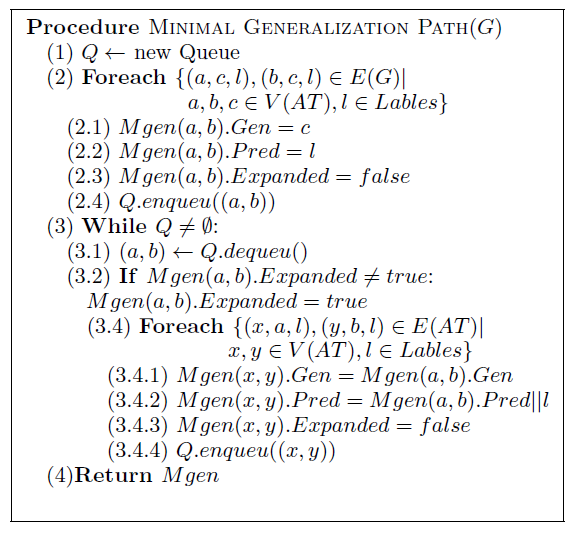
\includegraphics[width=0.7\linewidth]{diagram/minGeneralisation}
	\caption{Procedure of calculating minimal generalisation path \citep{radinsky2012learning}}
	\label{fig:mingeneralisation}
\end{figure}
\vspace{-1.5cm}

\subsubsection{Semantic Network}
Semantic network is a graphical knowledge representation in pattern of interconnected nodes. It stores knowledge in the form of semantic triple, where are subject-predicate-object. For example, \cite{kaschesky2011opinion} had developed SenticNet that collect sentiment from users whenever they express positive or negative feelings on writing comments or reviews online. In this study, World ontology will be used as reference semantic network. It models places and political entities of the planet Earth and linked data from Wikipedia, ConceptNet, WordNet, Yago and OpenCyc. World Ontology is used in generalisation as it generalise similar object. For example, Paris and London will be categorised under 'Capital' and connected to the node of 'Europe' in World ontology. By referring semantic network, knowledge obtained from the model is realistic.  

\subsubsection{Clustering Algorithm}
Clustering is a process to divide huge volume of data into number of groups in such that each group have the most similarity than those in the other group. \citep{sauravkaushik2016}. Clustering is important for identifying the characteristics of unstructured data and tag them with corresponding category. There are commonly four type of clustering, which are hierarchical, distance-based partitioned and organizing map algorithm. \citep{suyal2014text} 

\begin{enumerate}
\item \textbf{Hierarchical Clustering}

Hierarchical clustering uses the concept of successively merging each data into predefined cluster based on their similarity. It is represented by nodes and connectors and a sample of hierarchical cluster is illustrated in Figure 2.11. There are two types of hierarchical clustering, agglomerative and divisive. Agglomerative is a bottom-up approach which the algorithm starts with a single objects as separate category and repeatedly merge with another similar category until meeting stopping condition. Divisive is a top-down approach in which the algorithm start with one cluster and splitting recursively into branches.  
\vspace{-1cm}
\begin{figure}[H]
\centering
\fbox{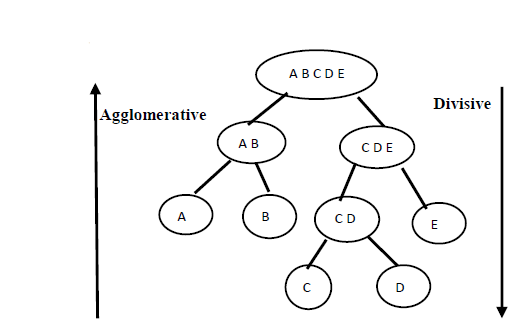
\includegraphics[width=90mm,scale=0.5]{./diagram/cluster1}}
\caption{Hierarchical cluster \citep{suyal2014text}}
\end{figure}
\vspace{-1cm}
From Figure 2.11, for agglomerative (bottom-up) approach, unweighted pair group with arithmetic mean (UPGMA) is used to calculate the mean distance of elements. Given 2 cluster A and B, the mean distance in UPGMA is measured using 
\begin{equation}\label{2.2}
 \frac{1}{|A| . |B|} \sum_{x\in A}^{}\sum_{y\in B}^{}d(x,y)
\end{equation}
where $d(x,y)$ is the updated mean distance between two elements. After that, each $d(x,y)$ is stored into matrix to find the smallest value of D and merge both elements using the smallest value of D into single cluster. 

The advantages of hierarchical clustering is simplicity, flexibility and use similarity as measurements while its disadvantages is that stopping condition is hard to obtain. In the study, hierarchical clustering will be used because abstraction tree (AT) is produced with adoption of causality graph. 

\item \textbf{Distance-based Partitioned Clustering}


This type of clustering make use of distance measurements to classify homogeneous data. Depart from hierarchical clustering, the problem of local minima that caused by branches of hierarchical cluster can be eliminated. K-mean clustering is one of the example that used Euclidean distance to calculate the nearest mean between two clusters. Figure 2.12 illustrated sample of K-mean clustering algorithm that differentiate different cluster according to their similarity and plot onto the graph. K-mean cluster different category of objects by the general formula of 
\begin{equation}\label{2.3}
	J = \sum_{j=1}^k\sum_{i=1}^n || x_i^{(j)} - c_j ||^2
\end{equation}
where J is the K-mean function, $\sum_{j=1}^k$ is number of cluster, $sum_{i=1}^n$ is number of case and $|| x_i^{(j)} - c_j ||^2$ is the distance function involving centroid for cluster j and case i.
\begin{figure}[H]
\centering
\fbox{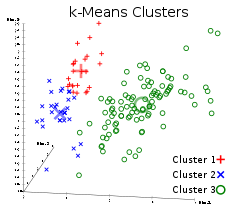
\includegraphics[width=70mm,scale=0.5]{./diagram/cluster3}}
\caption{K-mean clustering}
\end{figure}
\vspace{-1cm}
\item \textbf{Organizing Map Algorithm}

Self-organising maps (SOM) algorithm is one of the organizing map algorithm that produce low-dimensional regular grid and can be effectively utilized to visualize and observe characteristics of data. \citep{vesanto2000clustering}. SOM use concept of neural network with neuron and neuron weights are adjusted based on their features towards "winning" neurons. Figure 2.13 shows a visualisation of SOM. Self-organizing map describes a mapping from a higher-dimensional input space to a lower-dimensional map space. Once trained, the map can classify a vector from the input space by finding the node with the closest (smallest distance metric) weight vector to the input space vector. SOM comes with two major advantages, which are reducing data dimensions as SOM requires no target vector and without any external supervision and easily to classify based on data similarity. \citep{jaewookahnsueyeonsyn2005}

\begin{figure}[H]
\centering
\fbox{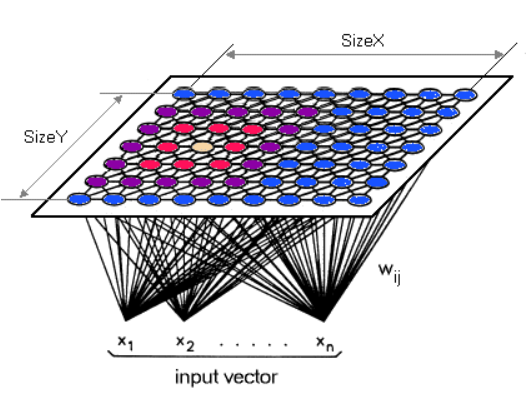
\includegraphics[width=100mm,scale=0.5]{./diagram/cluster2}}
\caption{Self-Organising Maps}
\end{figure} 
\vspace{-1cm}
\end{enumerate}




\section{Prediction Algorithm}
Prediction algorithm is an algorithm that modelling prediction and provides a guideline throughout the process of building up a predictive model. After obtaining extract keyword from textual data and clustering them based on clustering algorithm and relation extraction, the data is now said to be clean and sanitised. These clean data is then involve in prediction algorithm to build up a prediction model. 
\subsection{Sequential Prediction Algorithm}
Sequential prediction is a fast and simple pattern matching algorithm whereby comparing the past data or experience on a linear running timeline. There are many examples for sequential prediction algorithm such as medical condition that occur over time and patient conditions is getting either better or worse based on previous event. Besides, suggestion system that used in music application such as Spotify also involve in sequential prediction. 

\subsection{Neural Network Prediction Algorithm}
The biggest advantages of applying neural network in event prediction is the high tolerance and acceptance ability of noisy data and high accuracy. Despite of its complexity and long training time, many researches are more towards to neural network.\citep{granroth2016happens,hu2017happens,asencio2017medium}Neural network use the concept of brain metaphor for information processing and is suitable to discover previously unknown, valid patterns and relationship in large data sets. \citep{gaur2012neural}

\subsection{Decision Tree (Pundit) Algorithm}
Pundit algorithm is used in \cite{radinsky2014pundit} to learn and predict causality. It is one part of decision tree algorithm. Figure 2.15 shows the structure of Pundit algorithm and it started from extracting historical news article into causality pairs. Then, it generalises the pairs using causality prediction rules and create an abstraction tree for prediction. When a new event come in from world ontology , the events will compare the bottom node in the abstraction tree with similarity and after rounds of comparing, an effect event is produced and take as predicted event. Due to the highly flexible and fix with causality from news article, this study will focus on using Pundit algorithm to predict the future events. 

\begin{figure}[h]
\centering
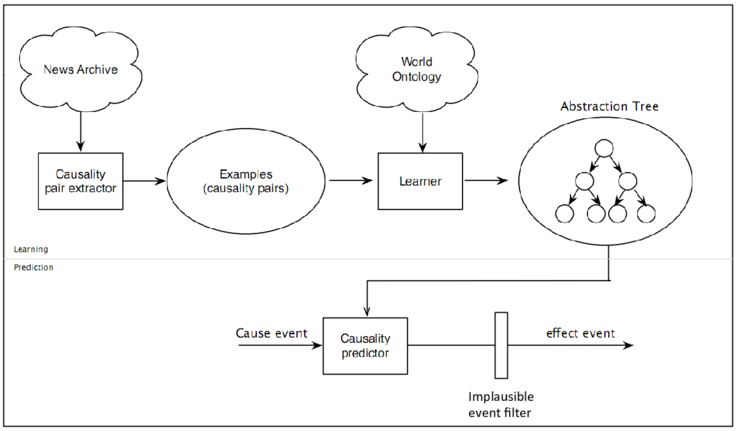
\includegraphics[width=1\textwidth]{./diagram/pundit}
\caption{Structure of Pundit Algorithm \citep{radinsky2014pundit}}
\end{figure} 
\vspace{-1cm}
From causality graph, the cause events will proceed to propagation in the abstraction tree to produce the predicted event. Figure 2.16 shows the propagation of cause event. The algorithm hold possible matched results in the abstraction tree (AT) and queue (Q) that act as search frontier. When the cause event searches AT using Q, the algorithm test the similarity of new cause event with parent node and if it meets the similarity score, the possible result is added and discuss on the accumulatively in final result.  

\begin{figure}[H]
	\centering
	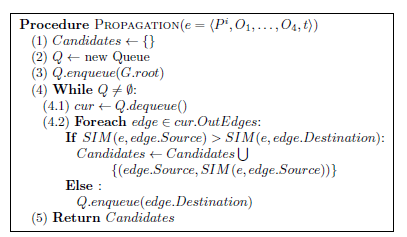
\includegraphics[width=0.7\linewidth]{diagram/propagate}
	\caption{Procedure for locating candidates for predictions \citep{radinsky2014pundit}}
	\label{fig:propagate}
\end{figure}
\vspace{-1cm}
For example, given an event of a bombing in Baghdad as input event illustrated in Figure 2.17, the input events search for the least general cause event that obtained in the past and eventually obtain te predicted result. 
\begin{figure}[H]
	\centering
	\fbox{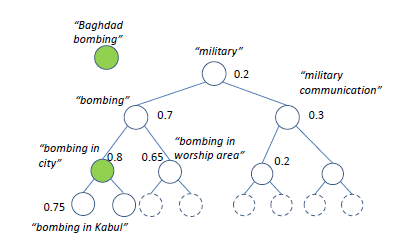
\includegraphics[width=0.7\linewidth]{diagram/abstractionTree}}
	\caption{Procedure in predictve model for input event of bombing in Baghdad \citep{radinsky2014pundit}}
	\label{fig:abstractiontree}
\end{figure}
\vspace{-1cm}



\section{Existing work of Event Prediction}

\begin{table}[]
	\vspace{-1cm}
	\centering
	\caption{Existing work on Event Prediction}
	\renewcommand{\arraystretch}{1.2}
	\noindent\makebox[\textwidth]{
		\begin{tabular}{|p{3cm}|p{3cm}|p{5cm}|p{4cm}|}
			\hline
			\textbf{Author, year} & \textbf{Work}                                                                                                                     & \textbf{Method}                                                                                                                                                                                                                                                                                             & \textbf{Advantages/Limitation}                                                                                                  \\ \hline
			\citep{letham2013sequential}& Sequential event prediction  & Given a sequence past database to predict next event within a current event sequence & Rely on additional user input, supervised ranking algorithm which not suitable for less predictive power past events \\
			\hline
			\citep{mirza2014extracting}   & Temporal sentiment analysis and causal rules extraction from tweets for event prediction & Event prediction based on temporal sentiment and causality from tweets which are from the opinion of people & Sentiment from tweets is uncertain and may affect on the predictive output \\
			\hline
			\citep{ding2015deep}  & Depp learning on event-driven stock market prediction  & Extract news text with dense vectors and train with novel neural tensor network, provides prediction based on convolutional neural network & Outcome is more focus on statistical, less focus on financial news that affect the share price in the market\\
			\hline
			\citep{hu2017happens}  & Event Prediction using Compositional Neural Network Model    & Use word2vec to represent events and build a compositional neural network model for future event prediction & Multiple event chain in CNN models and limited to learning associations between pairs of events \\
			\hline
			\citep{li2018constructing}   & Narrative event evolutionary graph (NEGG) for script event prediction  & Extract narrative event chain from newspaper and construct NEEG based on the chain &  Require expert knowledge in deep learning to produce NEGG   \\
			\hline
			\citep{rumi2018crime} & Crime event prediction with dynamic features and matrix factorisation   & Dynamic features such as visitor entropy, visitor homogeneity, region popularity, visitor ratio and count, observation frequency is taken as measurement in crime event prediction & Different city have different crime data, result may be biased \\
			\hline
			\citep{dami2018news}   & News events prediction using Markov logic networks & Markov logic network represent complex events by first-order logic and binded with domain-specific causal rules. Web ontology language (OWL) perform causal inference to represent probabilistic knowledge & Domain-specific causal rule must be created precisely before further text processing \\     
			\hline                                                                                                 
	\end{tabular}}
\end{table}

There are several researchers research on the topic 
of event prediction based on causality attributes and combining different method on different domain. Table 2.4 shows the existing work of event prediction, focusing on textual data from different domain such as financial, social media, medical etc. 

In the previous works, trend of event prediction starts from sequential approach, transforms to deep learning and even involved in neural network model. Researchers found that deep learning and neural network model able to cope with the high variety of unstructured textual data. Besides, event extraction also slowly transform from data-driven approach into knowledge-drive approach which able to observe from the latest work of \cite{dami2018news} that using Markov logic network with knowledge-driven extraction approach. In addition, among these previous study, causality is the main attribute that concern by the researchers. In this study, causality will also be the main attribute by producing causality rules and causality graph. Advanced method like neural network and deep learning will not be considered in this study since it require expert knowledge. We use the concept of Pundit algorithm which is also effectively predict future events from news articles because of the simplicity of algorithm and large corpus size from news article.  


\section{Open Issues and Challenges}
Event prediction is important and useful for public to have better insight and quick response against event might happen. However, there is several issues and challenges need to be addressed in order to produce a perfect predictive model approaching human-thinking. The issues and challenges are: 
\begin{enumerate}
	

\item \textbf{Low performance of predictive model due to low resource scenarios}

For predictive model, it require as much data as possible to train and test its accuracy and improve any weakness that learning from bad data sources. However, one of the problem is that there are scenarios of low resource that the prediction model can obtain. For example, if the model receive data source that are unique and only few events occurs because of these, the predicted output might not be valid and match with human-predicted output. 

\item \textbf{Word Sense Disambiguation}

In textual data extraction, word sense disambiguation is an open problem that troubling in determine the sense of word used in a sentence. One of the significant example can be observe in differences between dictionaries. 
For example, the word "\textbf{bank}" has 3 different meaning according to Cambridge Dictionary. First, bank is indicated as financial organisation where people can invest or store money inside, second is sloping raised land along sides of river, third is related to row of similar things. There are 2 sentences, "The \textbf{bank} will not be open in Saturdays" and "the river overflowed the \textbf{bank}.". The ambiguity between 2 same words but different meaning make machine difficult to detect and extract correct information from its true nature.

\item \textbf{Pronoun Resolution}

Pronoun resolution also known as anaphora resolution, is an common problem of resolving what a pronoun, or a noun phrase refers to. \citep{poesio2016anaphora}. Taking example of "John helped Mary", followed by "He was kind". As normal human, we can understand that "he" is indicating to John but not the machine. Machine will automatically define "he" as a new character instead of combining John with "he". Anaphora resolution is still an active research \citep{choi2016coreference,bandaragoda2018text} which contributes to better machine learning technique. 

\end{enumerate}
\section{Summary}
In this literature review, concept of event prediction and South China Sea conflict is clearly explained before moving in brief stage of event prediction. Then, stages within event prediction such as text mining, clustering, event relation extraction, prediction algorithm and etc is mentioned with details in the previous subchapter. Finally, this chapter discuss about previous and existing work that done by other researchers on the textual data event prediction in different domain and also the open issues and challenges in event prediction so that reader get better understanding about constraints of event prediction nowadays. 



% Chapter 3
\chapter{Research Methodology}

\section{Overview}
This study focuses on the implementation of abstract event causality networks proposed by \cite{zhao2017constructing} on South China Sea conflict. In this causality network, causality relation between events will be focused. This chapter emphasises the research framework of the study which explains the method and technique used to achieve the objective of the study. This chapter begins with the overview of research framework which consists of three phases and each phase will be briefly explained. Besides, overall research plan will be provided in order to give a better understanding on overall expected result of this study. After that, the chapter continues with brief description of data set which will be used in this study. Finally, the chapter ends with summary. 

\section{Research Framework}
\begin{figure}[H]
	\centering
	\includegraphics[width=1.0\linewidth,height=0.9\textheight]{"diagram/Research Framework"}
	\caption{Research Framework}
	\label{fig:research-framework2}
\end{figure}

The research framework consists of three phases which correspond to the three research objectives in Chapter 1. The three phases are; (i) Causality data corpus building based on South China Sea conflict news article, (ii) Construct abstract causality network using causal event extraction and generalisation, (iii) Causality network embedding model. The flow of these three phases is illustrated on the research framework in Figure 3.1.

In phase 1, news event will be represented in <cause, effect> format where it is named as causality pairs. Data is collected from various online news article that concerned on South China Sea conflict within China and Vietnam. After data collection, the following steps is causality mention extraction. Causality mention extraction will use specific causality connector such as "because", "because of", "after", etc to extract sentences that contain causality event. After that, "cause" and "effect" sentence will be extracted based on the template of <Pattern, Constraints, Priority> in order to clearly identify "cause" and "effect" sentence. Finally, event is represented in the causality pairs format of <Cause, Effect>. 

In phase 2, abstract causality network will be generated. <Cause, Effect> causality pairs from phase 1 are further extracted by using verb-and-noun representation. Verb-and-Noun representation is used because it preserve most of the important information rather then losing them. After extracting important information, the words is further generalised using WordNet and VerbNet. Each noun is generalised to its hypernym in WordNet while each verb is generalised to its class in VerbNet. Furthermore, frequently co-occurring word pairs (FCOPA) is used to identify the frequent term and will be represented as node of abstract causality network. The edges of causality network is constructed if there is existing edge in specific event. 

In phase 3, prediction model based on causality network embedding model will be proposed. Dual cause-effect transition (Dual-CET) model will be used for adopting essential characteristics of event causality such as asymmetry, transitivity and many-to-many. Besides, a ranking criterion will be used in order to learn the correct event embedding based on true causality pairs. Next, the Dual-CET model is measured by several evaluation criterion such as Random, Common neighbours, Jaccard's coefficient, etc to measure the effectiveness and reliability of the model.  
  
In addition, the main purpose of overall research plan is to provide a clear idea solve each research question that based on research objective, associated with its methodology and expected result.The overall research plan is tabulated in Table 3.1. In the first objective, the expected result should extracted keywords from South China Sea conflict-related news article in China and Vietnam as well as extract the causality connectors and represent them in causality pairs of <cause, effect> format. Meanwhile, in phase 2, the causality pairs will be further processed with causal event extraction and generalisation and visualise the causality network with nodes and edge based on processed causality pairs. Lastly, in phase 3, the study will focus on proposal of predictive model, which consist of building abstract causality network with frequently co-occurring word pairs (FCOPA) and embed the network with Dual-CET model. 

	\begin{table}[]
		\vspace{-1cm}
		\small
		\centering
		\caption{Overall Research Plan}
		\renewcommand{\arraystretch}{1.5}
		\noindent\makebox[\textwidth]{
	\begin{tabular}{|p{3cm}|p{3cm}|p{4cm}|p{4cm}|p{3cm}|}
		\hline 
		Research Objective & Research Question & Methodology & Result & Performance Measure \\ 
		\hline 
		To extract <cause, effect> causality pairs from news articles in South China Sea conflict by using causality connectors 
		& How to obtain useful information from news article that related to South China Sea conflict?  
		& 
		\begin{minipage}[t]{\linewidth}
			\begin{itemize}
				\item Build news article corpus of SCS conflict from online news article that focus on issues within China and Vietnam 
				\item Extract causality pairs of <cause, effect> using causality connectors based on template of <Pattern, Constraints, Priority> 
			\end{itemize} 
		\end{minipage}
		& 
		\begin{minipage}[t]{\linewidth}
				\begin{itemize}
				\item News article on South China Sea conflict within Vietnam and China is extracted and created news corpus.
				\item Event is extracted and represented in <cause, effect> causality pairs format. 
			\end{itemize} 
		\end{minipage}
	
		& Make sure event pairs is represented in <cause, effect> format \\ 
		\hline 
		To extract all important information from causality pairs by using verb-noun representation as well as discover general patterns using WordNet and VerbNet. 
		& How to generalise and cluster event extraction and how to relate event pairs with causality? 
		& 
	 	\begin{minipage}[t]{\linewidth}
 			\begin{itemize}
 			\item Extract all the important information within causality pairs by using verb-noun representation.
 			\item Generalise all the verb and noun with WordNet and VerbNet. 
 		\end{itemize} 
	 	\end{minipage}
		& 
		\begin{minipage}[t]{\linewidth}
		 \begin{itemize}
			\item All the important information will be kept while eliminating unused information.  
			\item All information is generalised to produce a general, frequent and simple causality patterns. 
		\end{itemize}
		\end{minipage}
		& Visualise causality network with nodes and edge \\ 
		\hline 
		Train and build an abstract causality network with frequently co-occurring word pairs (FCOPA) and embed the model into a continuous vector space. 
		&How to use the extracted information to train and build a prediction model?
		&
		\begin{minipage}[t]{\linewidth}
			\begin{itemize}
				\item Build abstract causality network with frequently co-occurring word paris (FCOPA)
				\item Embed causality network with Dual-CET model.
			\end{itemize}
		\end{minipage}
	 	& 
		\begin{minipage}[t]{\linewidth}
			\begin{itemize}
			\item Prediction model will be generated and able to generate general predicted output based on inputted event.
			\item Accuracy of prediction model is measured.  
			\end{itemize}
		\end{minipage}
	 	 & 
		Examine prediction model by performing several evaluation criterion such as Random, Common neighbours, Jaccard's coefficient.\\ 
		\hline 
	\end{tabular}} 
\end{table}


\subsection{Phase 1}
Phase 1 is causality data corpus building and it is important to convert unstructured data from news article to structure form and understandable by the computer. There are several steps to build up a good data corpus which involve specific data collection, causality mention extraction and event representation.
\begin{enumerate}[label=(\alph*)]
	\item Data Collection
	
	The data is collected from news article based on keyword of South China Sea conflict such as "South China Sea", "ASEAN", "Spratly", "Island", "People's Court",etc. In the news article that consist of these keywords, these articles are taken according to the country where the news being published. This will be further explains in the subsection of data set. 
	
	\item Causality Mention Extraction
	
	In causality mention extraction, the selected news article is then further selected with causality connectors such as "because", "because of", "after", "therefore", "lead to", etc. First of all, sentence segmentation will be used to split all of the sentence in the article. Then, all of the sentence is filtered by causality connectors. After that, regular expression (Regex) will be used to setup extraction rules and pattern and return the result of "cause" and "effect". 
	 
	\item Event Representation
	
	In event representation, causality pairs format will be used as each sentence is represented as \textit{<Cause, Effect>}. This representation can be done from obtaining the value based on the pattern of regular expression. For multiple data that obtained in multiple article, all the causality pairs is stored in JSON format. 
	
\end{enumerate}
\subsection{Phase 2}
Phase 2 is discussing about abstract causality network by using causal event extraction and generalisation. After obtaining causality pairs, the pairs still needed to be further processing in order to obtain useful information. At this stage, both cause and effect triple is now in sentence form. In order to obtain and preserve all the information within the triple, verb-and-noun representation is used. After that, all the verb and noun within the triple are generalised using WordNet and VerbNet. Then, the specific causality network is build by using these information. In order to obtain a frequent, general causality pattern, the causality pair is then generalised with frequently co-occurring word pairs (FCOPA) to build up abstract causality network. 

\begin{enumerate}[label=(\alph*)]
	\item Causal Event Extraction
	
	For shrinking down the causality pairs that obtained from the previous steps, causal event extraction is needed. First, POS tagging is used to tag out all the words with their unique characteristics. Then, for each verb, noun and proper noun will be taken and update the triple. Meanwhile, the remaining words will be removed. 
	
	\item Causal Event Generalisation
	
	After extraction, there are still a lot of redundant and similar words within the triple. Hence, generalisation is needed. By using WordNet, noun and proper noun will be generalise to their synonym or hypernym while verb will be generalised to its class by using VerbNet. 
	
	\item Abstract Causality Network
	
	
\end{enumerate}
\subsection{Phase 3}
Phase 3 is to implement and train the predictive model as well as filter any inappropriate output. In machine learning, a model that generated needs to be trained as the model will dynamically learn the pattern from the inputs and fix any error that occurred during its training. In this study, a new cause event will act as input and predicted effect events will act as output. While adding the input cause event into the model, steps need to be taken as guideline for the overall event prediction.  
\begin{enumerate}[label=(\alph*)]
	\item Train prediction Model
	
	In this study, Pundit algorithm is used to predict desired effect events based on previous knowledge obtained. In training the prediction model, first the input cause events need to propagate throughout the abstraction tree to obtain a set of matched node. After obtaining matched nodes, causality prediction rules and minimal generalisation path that generated in the previous steps are used to guide the input cause event in finding the similar effect events. As a result, predicted effect event is produced. 
	 
	\item Pruning Implausible Effect
	
	Before giving the most suitable prediction, filtering process needs to be taken as the system might produce implausible effect events which leads into false prediction. Point-wise mutual concept information (PMCI)
	\begin{equation}\label{3.2}
	PMCI(x,y) = log \frac{P(x,y)}{P(x) | P(y)} 
	\end{equation}where x is the cause event and y is the effect events. By measuring PMCI, the model filter the predicted effect events that have low average PMCI.  

\end{enumerate}
\section{Data sets}
This study will focus on South China Sea conflict news article from online resource within China and Vietnam. Keywords such as "China", "Vietnam","South China Sea", "Spratly", "World Court" will be used to search online news article. Once the news article matched with the keywords, it is taken as our data sets for further data processing.The collected data is then grouped according to corresponding country based on the location of the news published. For example, if the news are published in Hanoi, the news is grouped into Vietnam since Hanoi is one of the state in Vietnam. In this study, only 30 online news from China news agency and 30 online news from Vietnam news agency will be taken. In Figure 3.2 and 3.3, sample of news article from Vietnam and China is taken from online resources and put into .txt document file.          
\begin{figure}[H]
	\centering
	\fbox{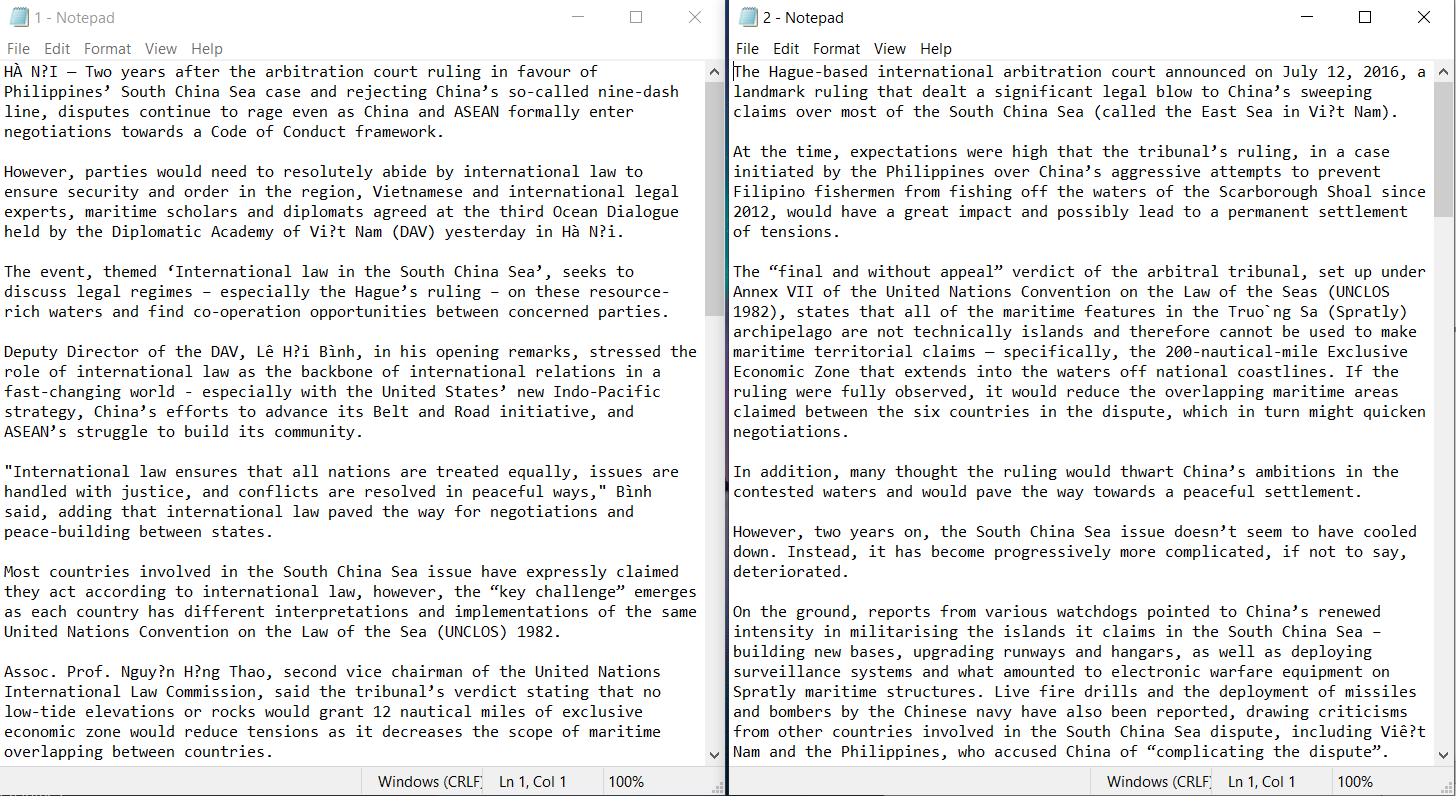
\includegraphics[width=1.0\linewidth]{diagram/vietnamNews}}
	\caption{Sample of news article from Vietnam New Agency}
	\label{fig:vietnamnews}
\end{figure}
\vspace{-1cm}
\begin{figure}[H]
	\centering
	\fbox{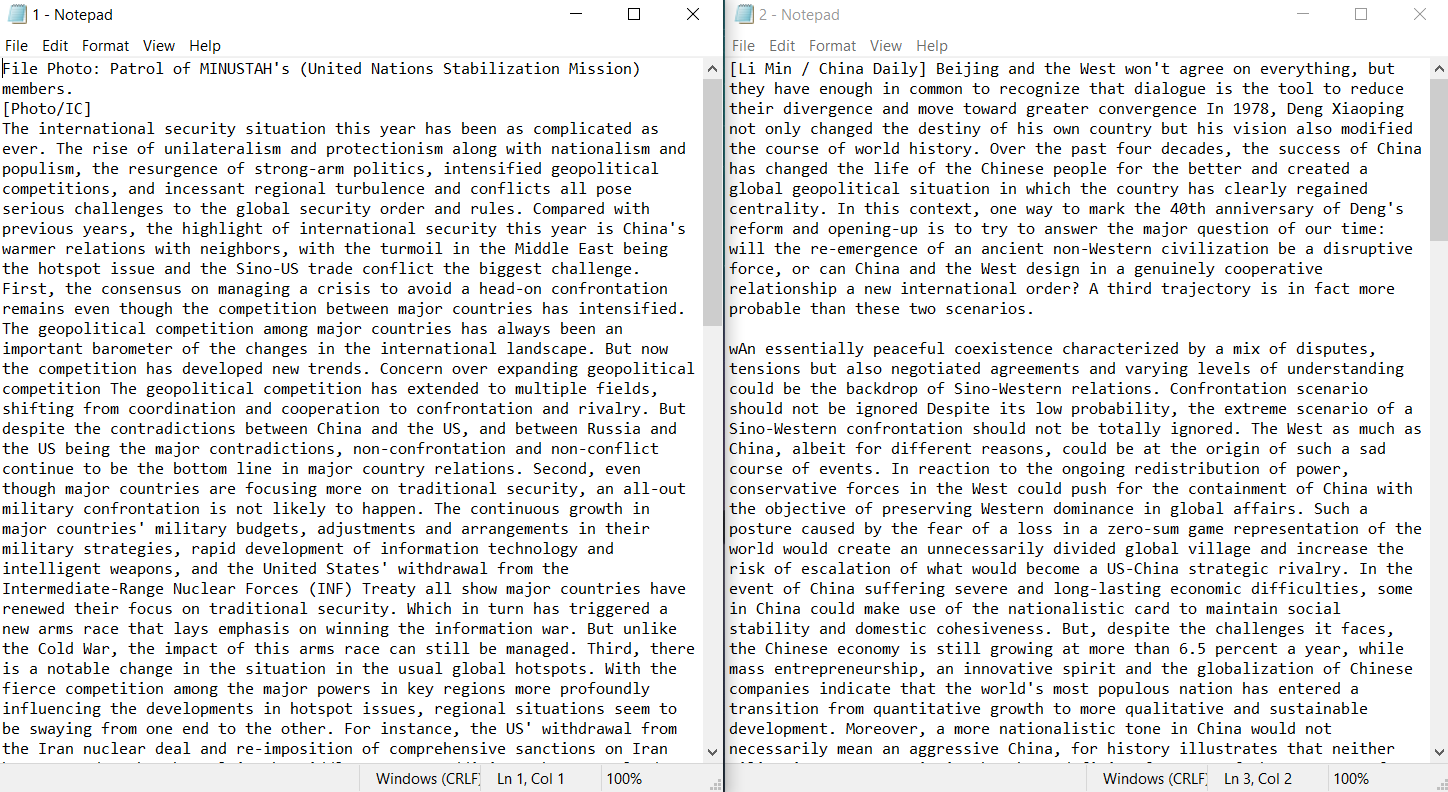
\includegraphics[width=1.0\linewidth]{diagram/chinaNews}}
	\caption{Sample of news article form China}
	\label{fig:chinanews}
\end{figure}
\vspace{-1cm}
To clean the data set, this study will used WebAnno annotation tool to manually annotate keywords based on corresponding entities. After that, stemming process will be taken to reduce verb into its basic form. Finally, these corresponding entity based on different word characteristics are grouped them into 5 tuple of <Actor, Action, Object, Location, Object>. 


\section{Performance Measurement}
To measure the performance of the prediction model, precision and recall as well as F1-score are used. Confusion matrix in Figure 3.4 also provides classification of evaluation between actual event and predicted event.

\begin{figure}[H]
	\centering
	\fbox{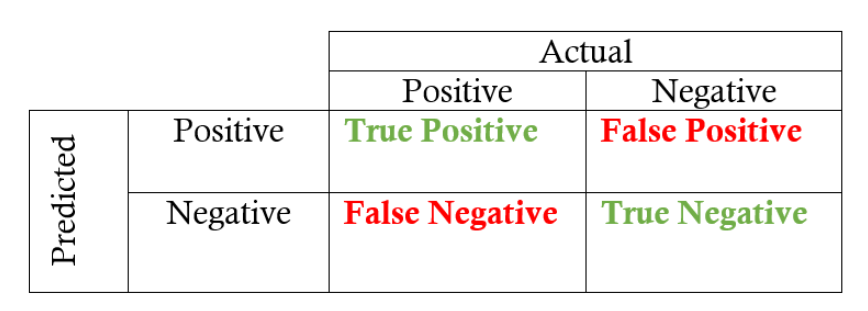
\includegraphics[width=0.7\linewidth]{diagram/confusionMatrix}}
	\caption{Confusion Matrix}
	\label{fig:confusionmatrix}
\end{figure}
\vspace{-1cm}

Precision is the percentage of relevant results while recall is the percentage of total relevant result that correctly identify from prediction model. Both formula of precision and recall are
\begin{equation}\label{3.3}
\textbf{Precision} = \frac{True Positive}{Actual Results} 
\end{equation}
\begin{equation}\label{3.4}
\textbf{Recall} = \frac{True Positive}{Predicted Results} 
\end{equation}
To summarise the usage of precision and recall, F1 score is used to give a higher priority to maximizing precision and recall to the prediction model. F1 score is formulated from 
\begin{equation}\label{3.5}
\textbf{F1 score} = 2 * \frac{Precision * Recall}{Precision + Recall} 
\end{equation}

\section{PSM 1 Gantt Chart}
The PSM 1 Gantt Chart is in Appendix A. 

\section{Summary}
Chapter 3 discussed the method and steps to use throughout the project. In Research Framework, each of the phase will generate important output and consecutively become input for the next phases. For phase 1, data corpus is built from unstructure textual data from SCS-related news article and represent in 5 tuple format. Then, in phase 2, the sanitised event are generalised and an abstraction tree is built by using HAC hierarchical clustering. Causality prediction rules is also generated in order to generate predicted effect events. Finally, in phase 3, prediction model is trained and the output is filtered in order to produce high quality and reliability output. The prediction model is then evaluate by performance measurement such s precision and recall. Data set used in this study are also stated as it is the main source for this project.  


%Chapter 4
\chapter{Experimental Setup}
\section{Introduction}
In this chapter, an experimental setup is done by working on phase 1 in the Research Framework. Steps in Phase 1 such as data collection, text preprocessing and event representation will be explained in details. After that, this chapter displays the initial result and finding of phase 1. Finally, the chapter ends with a summary of the chapter.

\section{Text Preprocessing and Event Extraction}
In phase 1, the data is collected from online news article that is related to South China Sea conflict with the selected keywords. In order to present the process of text preprocessing, sample sentence is taken from one of the news article. The sample of sentences is \textit{"Two years after the arbitration court ruling in favour of Philippines’ South China Sea case and rejecting China’s so-called nine-dash line, disputes continue to rage even as China and ASEAN formally enter negotiations towards a Code of Conduct framework."}, taken from VietnamNews. In this sentence, we can obtain that the SCS disputes continue to rise as issues occur in SCS countries.

In phase 1, text preprocessing will be the primary work. Purpose of text preprocessing is to structure the unstructured textual data and extract useful information while ignoring those duplicated and meaningless words. There are few steps involved in text preprocessing such as annotation, stemming and representation. Figure 4.1 shows the flow of text preprocessing in phase 1.
\begin{figure}[H]
	\centering
	\fbox{\includegraphics[width=0.8\linewidth]{"diagram/phase1 steps"}}
	\caption{Flow of Text Preprocessing}
	\label{fig:phase1-steps}
\end{figure}
\vspace{-1cm}

At the beginning of the project, this project tend to extract information by using standard Named Entity Recognisation (NER). NER is a part of information extraction that identify named entity within a sentence.  However, standard NER has its limitation that only able to recognise person, organisation, location and time. Figure 4.2 shows the limitation of NER extraction by using sample sentence. 
\begin{figure}[H]
	\centering
	\fbox{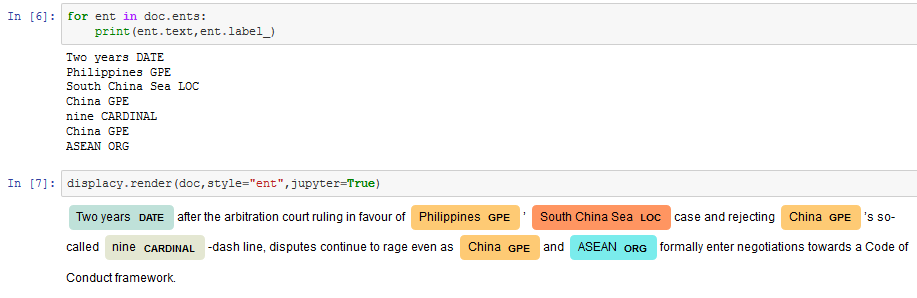
\includegraphics[width=1.0\linewidth]{diagram/spacy4}}
	\caption{Limitation of standard NER for only extracting person, organisation, location and time}
	\label{fig:spacy4}
\end{figure}
\vspace{-1cm}

Thus, manual annotation is used to annotate important entity such as action, object and instrument. For annotation, WebAnno annotation tool is used. WebAnno is a general purpose web-based linguistic annotation tool including various layers of morphological, syntactical and semantic annotations. By using WebAnno, this study is able to add custom entity and annotate them with matched words. Figure 4.3 shows annotation of sample sentence in WebAnno. 
   
\begin{figure}[H]
	\centering
	\fbox{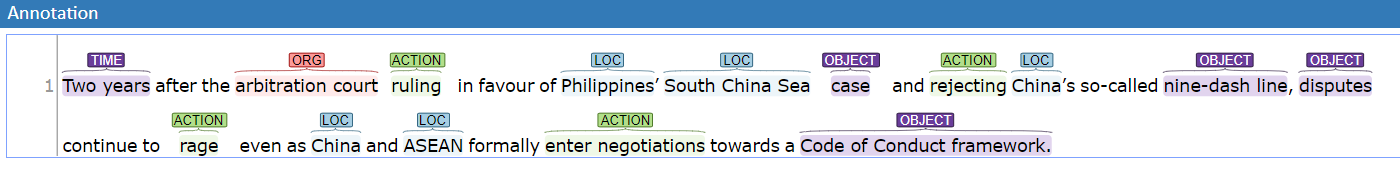
\includegraphics[width=1.0\linewidth]{diagram/annotation}}
	\caption{Annotation of sample sentence in WebAnno}
	\label{fig:annotation}
\end{figure}
\vspace{-1cm}
After annotation, the output is printed using CoNLL-2002 format. CoNLL-2002 format is a data output format which consists of two columns separated by a single space. There are 2 attributes in CoNLL-2002. The first one is tag format which B denotes first item and I denotes non-initial words. The second one is the entity tag of the words. Figure 4.4 shows the CoNLL-2002 data output of annotation. In this format, the custom entity such as \textit{TIME}, \textit{ACTION} and \textit{OBJECT} will be defined accordingly. 
\begin{figure}[H]
	\centering
	\fbox{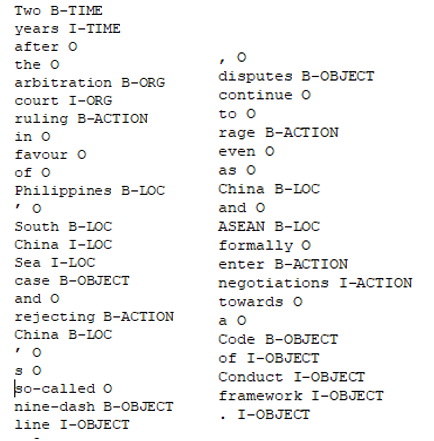
\includegraphics[width=0.9\linewidth]{diagram/annotationResult}}
	\caption{Annotation in CoNLL-2002 format}
	\label{fig:annotationresult}
\end{figure}
\vspace{-1cm}

After that, all the entity tag with \textit{ACTION} will be normalised through stemming. Stemming is the process where convert verb into its basic form. For example, in the sample sentence, "ruling" and "rejecting" are the entity tag with \textit{ACTION}. After stemming, they will become "rule" and "reject" respectively. In the following steps, these custom entity will be assigned into 5 tuple of <Actor, Action, Object, Location, Timestamp> for event representation. Both stemming and representation will be done in the future.  


\section{Summary}
In this chapter, the preliminary works in phase 1 is done on the data collected from South China conflict.First, the annotation model is preset with custom entity tag because there are limitation of entity in standard NER. The limited entity in standard NER are person, organistion, location and time which are required to have more in this study. Then, the annotation is then output as CoNLL-2002 format as it provides simple yet essential output for the further text processing. After that, the words with custom entity of \textit{ACTION} are stemmed into its basic form. Finally, these customer NER will be represented in 5 tuple approach. These preliminary works is important so that the following text processing will be successful and works on the right path.  

%Chapter 5
\chapter{Conclusion}
\section{Conclusion Remarks}
After performing preliminary task in previous chapter, the initial result had been partially achieved. Data source is cleaned and sanitised.  Cleaned data is suitable for further processing to obtain valuable information. However, there are a lot of works needs to be done in order to reach the stage of building up prediction model and it will be discussed in the next section. In this study, the main attributes is causality. Causality is used to indicate the relation between cause and effect. In the future works, this study needs to extract the causality from news article and compare with world ontology to get precise knowledge on the same domain. Besides, Pundit algorithm needs to be followed from step to step as a guideline in this study. Pundit algorithm provides a prediction framework that start from learning the causality of events until the prediction of future event. By obeying Pundit algorithm, the predicted effect event will have high reliability and precision. 

\section{Future Works}
After annotating entity from sample sentence in previous chapter, these entities need to be assigned based on their characteristic which manually defined by researcher. In addition, another challenge is to put all these entities into corresponding tuple <Actor, Action, Object, Location, Timestamp>. This step might require some recursive algorithm that constantly load matched entity into the tuple.

In the next phase, which is phase 2, the extracted tuples are being generalised in order to reduce the size of corpus. Generalisation is measured by using the similarity of the event pairs based on world ontology. By generalising the event pairs, multiple generalisation path will be created and the shortest path are defined as minimal generalisation path. With minimal generalisation path, an abstraction tree is built and the nodes within the abstraction tree is cluster through HAC hierarchical clustering. After that, causality prediction rules is set in the form of <Pattern, Constraints, Priority> for the preparation of input cause event to generate most possible effect event. 

In phase 3, the prediction model based on abstraction tree is built. Test data are taken from new input cause event and the new event will propagate throughout the abstraction tree to find the matched node. During the propagation, minimal generalisation path and causality prediction rules are used to guide the input events for the desired effect event. To maximize the performance of prediction model, filtering process will take place to eliminate inappropriate predicted effect event. Filtering process will be handled by PMCI calculation to match up the relativeness between cause and effect. Finally, performance measure by using precision and recall will be evaluated the accuracy and precision of the prediction model. 

\section{Summary}
This chapter discusses the overall conclusion and the future works that require completing within this project. After finishing the steps in previous chapter, there are still a lot of works need to be done, such as event generalisation, causality prediction rules generation, building up an abstraction tree, etc. Future work will be done on the following chapter and causality will be focus in this study so that event pairs has strong causal relation that satisfy the requirement of event prediction.  



\bibliographystyle{utmthesis-authordate}
\bibliography{reference}

\appendix
\chapter{PSM Gantt Chart}
\begin{figure}[H]
	\centering
	\includegraphics[angle=90,width=1.0\linewidth]{"diagram/Thesis Gantt Chart NEW"}
	\label{fig:thesis-gantt-chart-new}
\end{figure}


\endmatter
\end{document}
